Um die Sicherheit während der Benützung des Luftkissenboots zu gewährleisten, wurden mehrere Sicherheitsvorkehrungen getroffen. 
%Weiters wurde auch auf die Gerätesicherheit geachtet, siehe \autoref{sec:Geraetesicherheit}
\section{Sicherheitsmaßnahmen}
\subsection{Not-Aus--Schalter mit Schlüssel}
Das Betätigen des Not-Aus--Schalters führt zu einer Unterbrechung des Haltestroms für das Hauptrelais. Das heißt, das Relais fällt ab und unterbricht die beiden Akkustränge, was den Stromkreis öffnet.\\
Der Not-Aus--Schalter muss nach Betätigung mittels Schlüssel entsperrt werden.
%Die Notabschaltung der gesamten Elektronik erfolgt durch Betätigen des Not-Aus-Schalters, da dies den Haltestrom des Hauptrelais unterbricht. Der 
%Es ist möglich das Hovercraft nach einer Notabschaltung mit Hilfe des Schlüssels wieder zu starten. 
\begin{figure}[h]
    \centering
    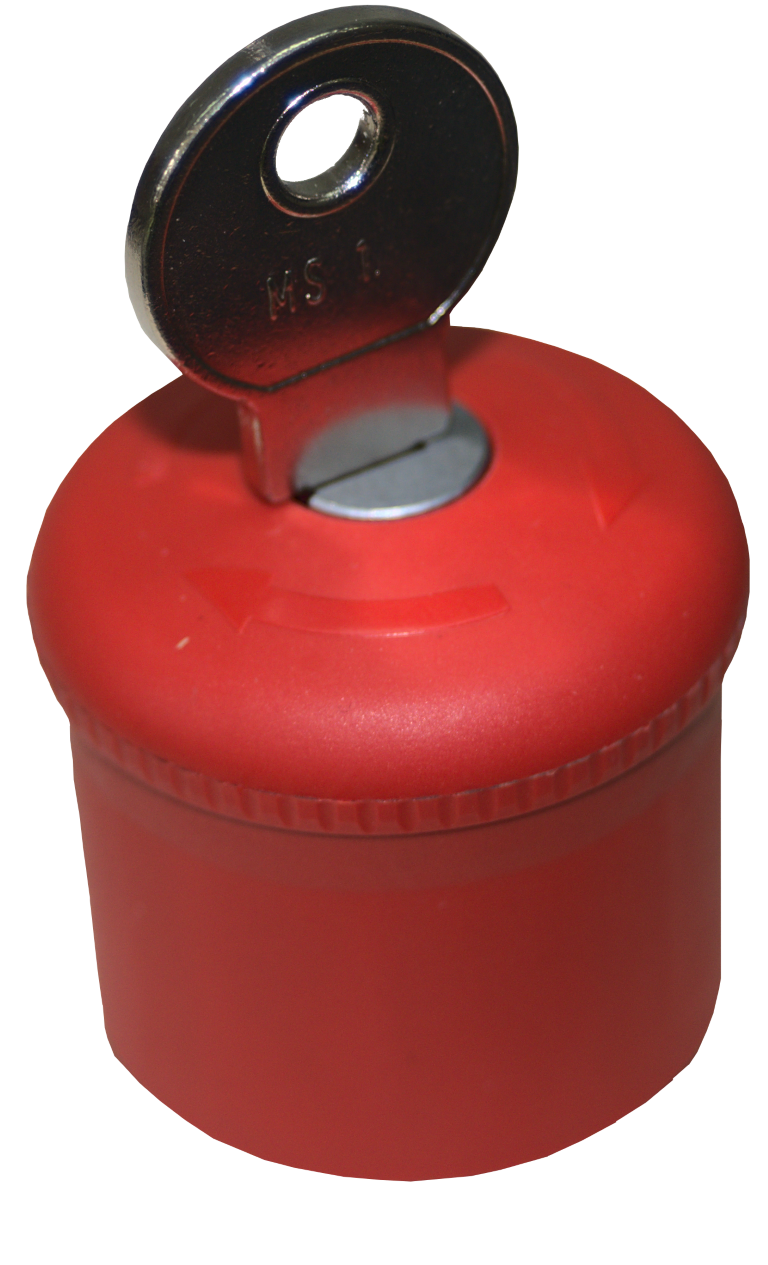
\includegraphics[width=0.35\textwidth]{Fotos/Notaus.png}
    \caption{Not-Aus--Schlüsselschalter}    
\end{figure}

\clearpage
\subsection{Daumengas für beide Propeller}
Die beiden Motoren werden durch zwei Daumengashebel am Lenker angesteuert. Sollte der Fahrer vom Lenker abrutschen, lässt er somit automatisch die Daumengashebeln los, was zu einem Bremsvorgang der Motoren führt.
%Durch Betätigen der beiden Daumengase, rechts und links am Lenker, erfolgt der Antrieb der Propeller. Das linke Daumengas ist für den Auftrieb, für den unteren Propeller und das rechte für den Antrieb, den hinteren Propeller. Durch Loslassen des Daumengases bremst das Hovercraft sofort.
\begin{figure}[h]
    \centering
    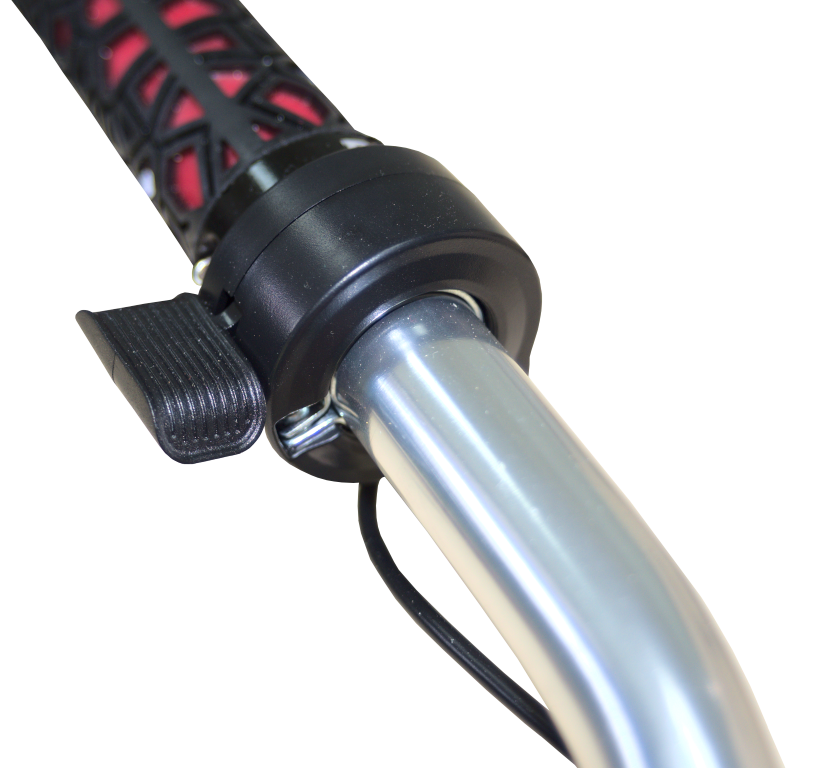
\includegraphics[width=0.65\textwidth]{Fotos/Daumengas.png}
    \caption{Daumengas}    
\end{figure}

\newpage
\subsection{Gitterabdeckungen}
Die beiden Propeller sind durch Gitter geschützt, die es unmöglich machen, unbewusst in ein drehendes Teil zu fassen. Das untere Gitter ist so konzipiert, dass es das Gewicht des Fahrers problemlos tragen kann.\\
Außerdem dienen die Gitter als Schutz vor losen Teilen (wie zum Beispiel Steinen), die sich in den Propellern verfangen könnten.
\begin{figure}[H]
    \centering
    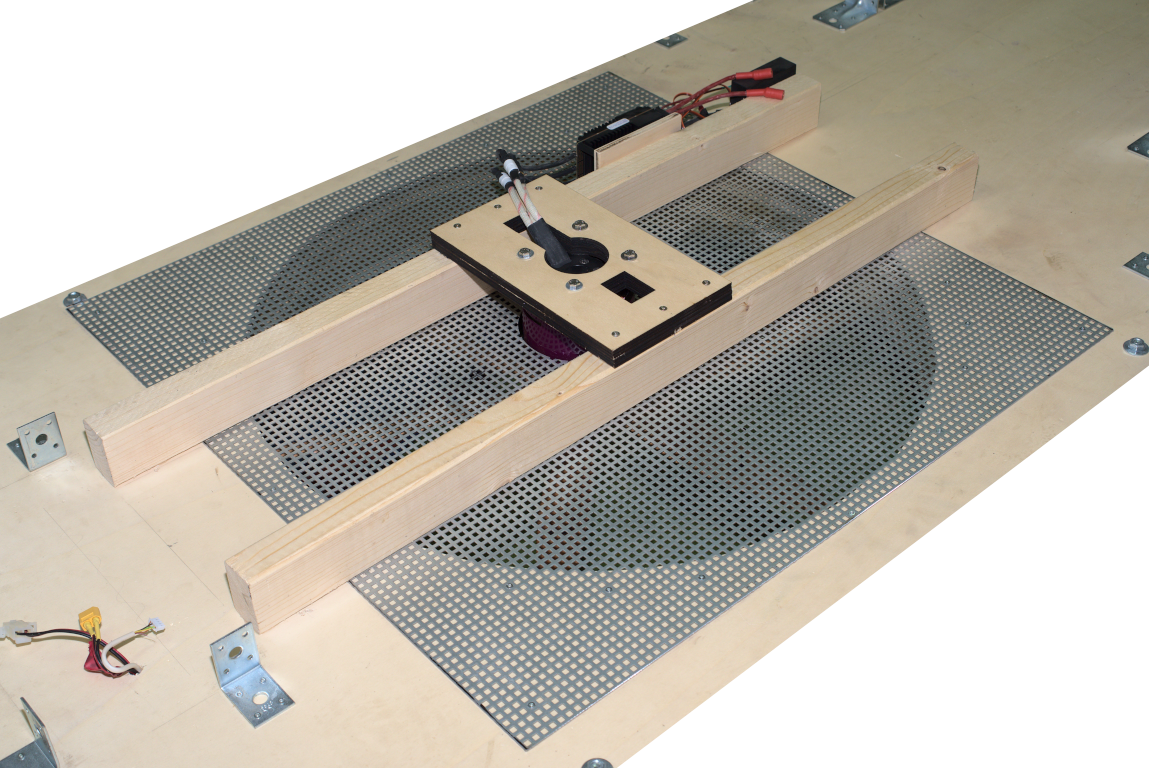
\includegraphics[width=0.75\textwidth]{Fotos/Konstruktion/DSC_8718_gitter_unten.png}
    \caption{Unteres Gitter}    
\end{figure}

\begin{figure}[H]
    \centering
    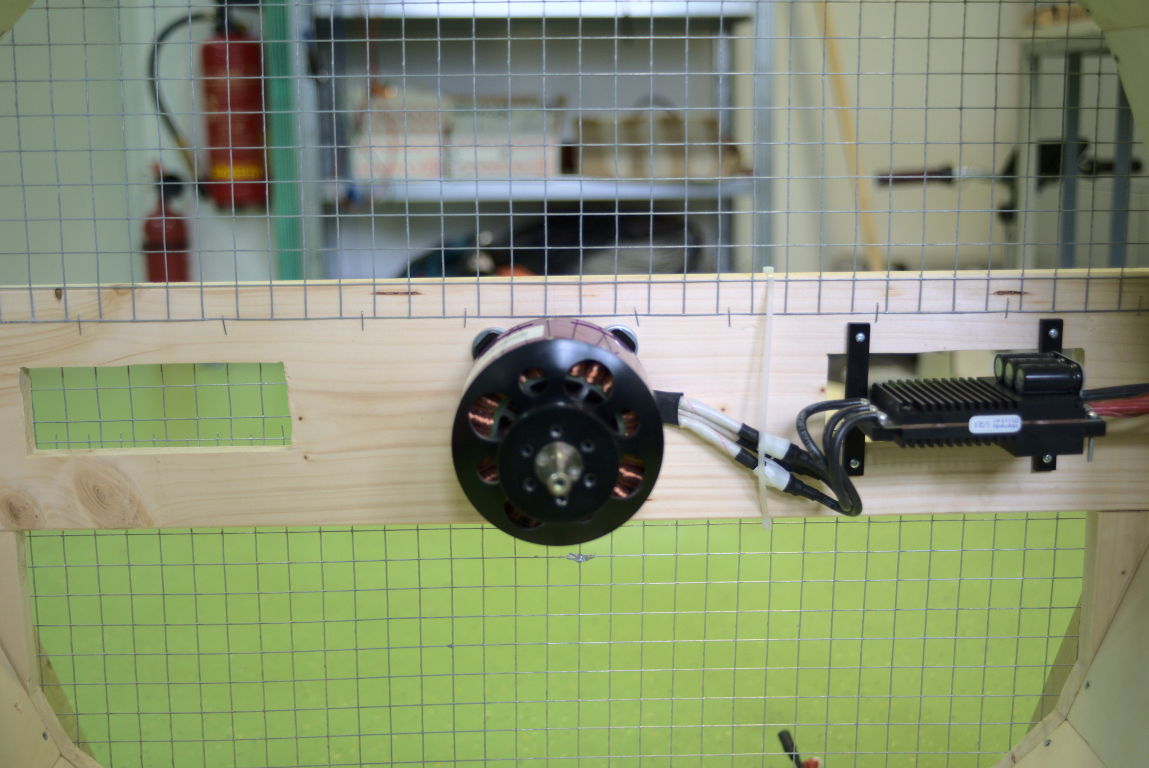
\includegraphics[width=0.75\textwidth]{Fotos/Konstruktion/DSC_8776_gitter_hinten.png}
    \caption{Hinteres Gitter}    
\end{figure}


\section{Gerätesicherheit \label{sec:Geraetesicherheit}}

\subsection{Ladevorgang}
Während des Ladevorgangs werden die Minuspole der beiden in Serie geschaltenen Akkustränge verbunden. Um den Kurzschluss eines Akkustranges zu verhindern, muss deshalb das Hauptrelais geöffnet sein.\\
Zum Schutz vor Bedienungsfehlern wurden Schalter in die Kabelbox verbaut. Diese unterbrechen bei offenem Deckel, und damit vorhandenem Zugang zu den Ladekabeln, den Haltestrom des Hauptrelais.\\
Trotz dieser Sicherheitsvorkehrung muss der Not-Aus--Schalter während des Ladevorgangs gedrückt sein.
% Während dem Ladevorgang wird es empfohlen, den Not-Aus betätigt zu haben, siehe \ref{sec:Anleitung_Laden}, um eine sichere Trennung vom Relais zu bieten. \\
% Weiters ist es notwendig, den Ladedeckel zu öffnen. Dies wird mithilfe von Schaltern überprüft. Falls der Ladedeckel offen ist, lässt sich das Hovercraft nicht starten. \\
% Das Hovercraft lässt sich auch laden, wenn der Not-aus nicht gedrückt ist. Dies ist aber nicht empfohlen!
\begin{figure}[H]
    \centering
    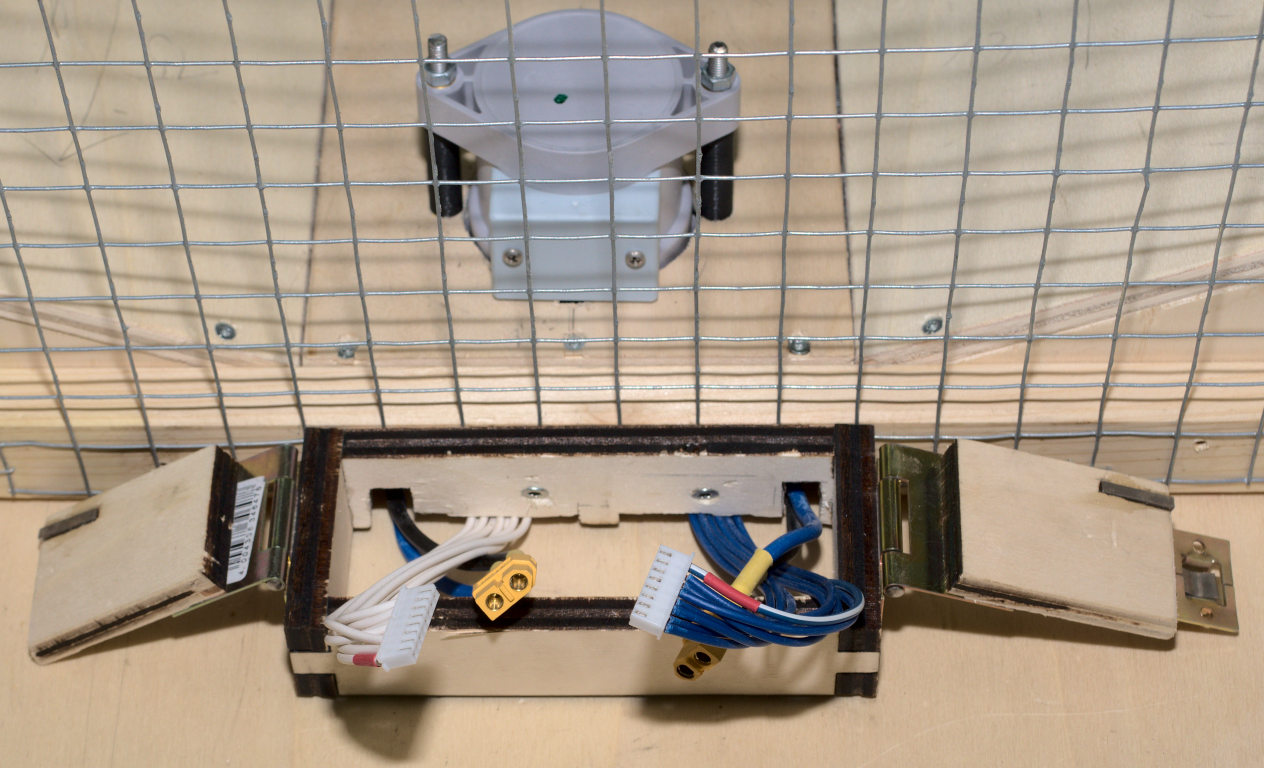
\includegraphics[width=\textwidth]{Fotos/Ladedeckel_DSC_8794.png}
    \caption{offene Ladebox \&\ Ladekabel \label{fig:offener_Ladedeckel}}    
\end{figure}

In der \autoref{fig:offener_Ladedeckel} sind die Endschalter noch nicht vorhanden, da sie erst zu einem späteren Zeitpunkt verbaut wurden. 

\clearpage
\subsection{Bremsschutz}
Zum Schutz des Schlauchbootbodens beim Bremsen wurde ein zusätzlicher Boden angebracht. Dieser wurde mit einem Kraftkleber und Lochband am Boot befestigt.\\
Der zusätzliche Boden bietet Schutz vor Abschürfungen, die während des Bremsvorgangs entstehen, und vor Steinen, welche das Boot zerstören könnten.
\begin{figure}[H]
    \centering
    \includegraphics[width=0.65\textwidth]{Fotos/Konstruktion/DSC_8616.png}
    \caption{Bremsschutz}    
\end{figure}

%\clearpage
\subsection{Reglerkühlung}
Die beiden Motorregler sind so positioniert, dass sie durch den vom Propeller erzeugten Luftstrom gekühlt werden. Außerdem schalten die Regler automatisch ab, sobald die innere Temperatur einen Schwellenwert von 90$^\circ$C überschreitet. 
%Die beiden Motorregler sind so positioniert, dass sie luftgekühlt und vor dem Überhitzen geschützt sind. Weiters haben sie auch eine automatische Abschaltung bei Übertemperatur eingebaut. Diese wurde auf $90^\circ C$ eingestellt. 
\begin{figure}[H]
    \centering
    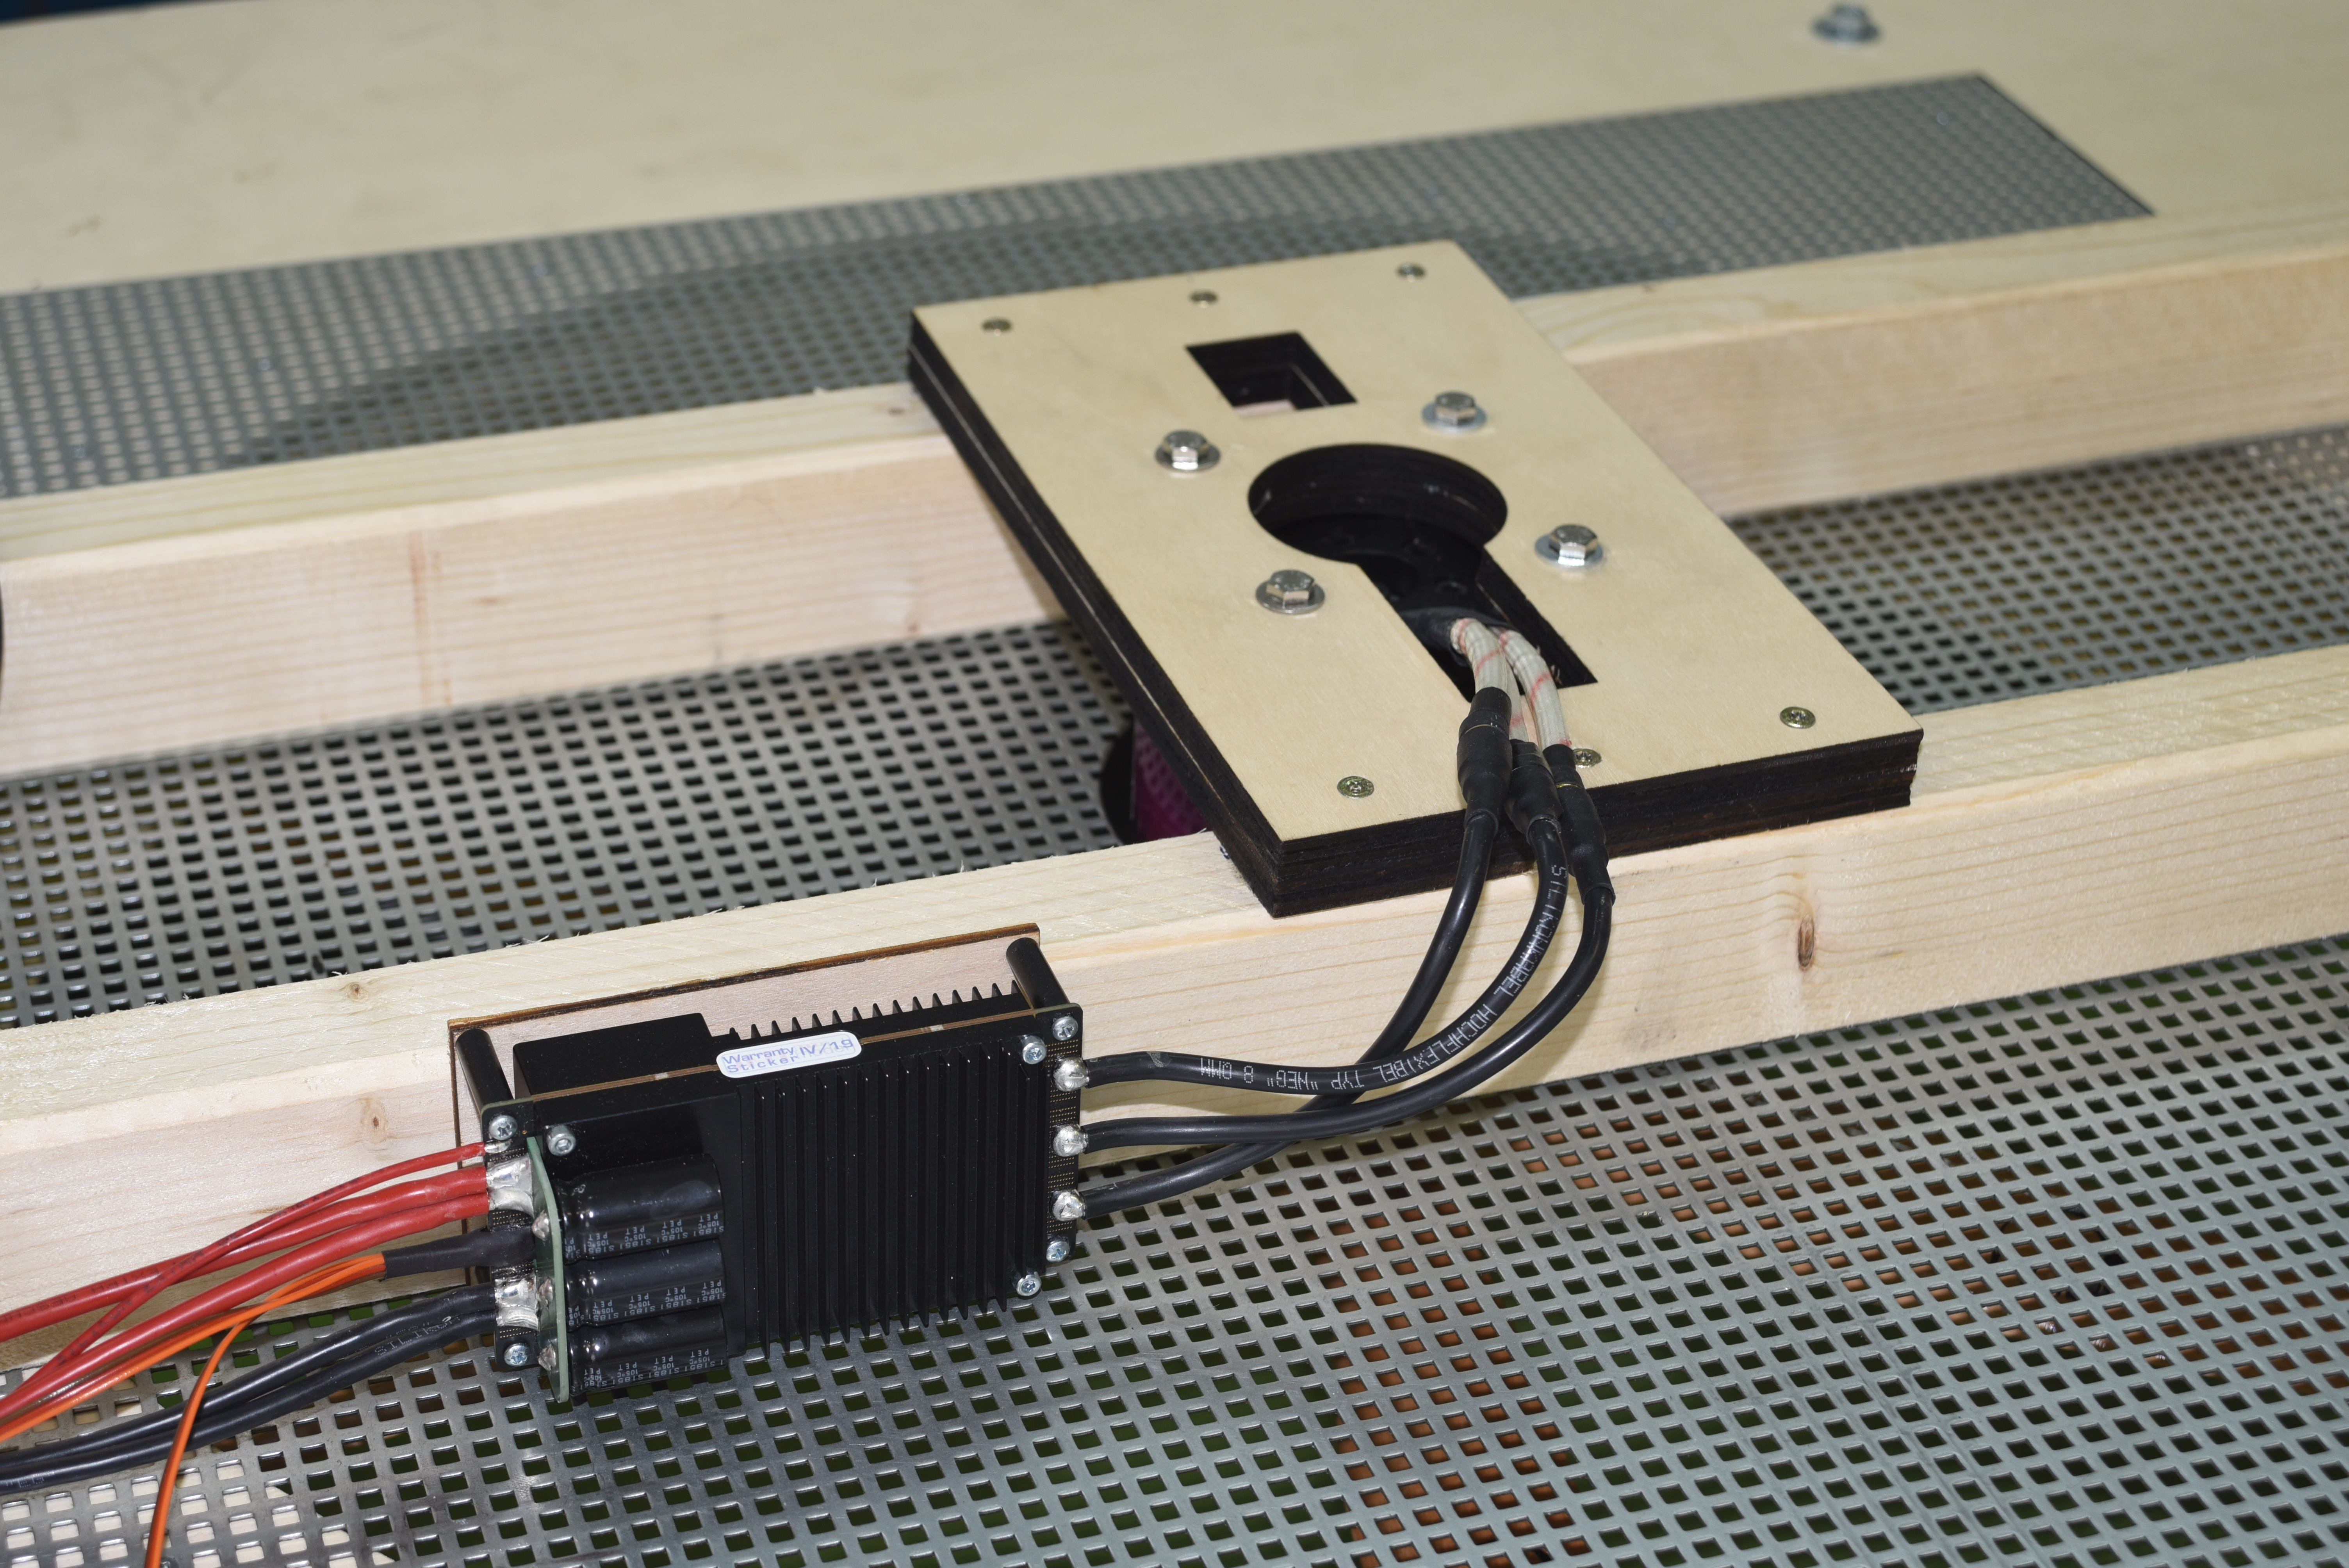
\includegraphics[width=0.65\textwidth]{Fotos/Gitter_unten.jpg}
    \caption{Position des Motorreglers}    
\end{figure}

% \subsection{KFZ-Sicherungen}
% Die KFZ-Sicherungen der Firma SIBA wurden eingebaut um die Akkus vor einem Kurzschluss zu schützen. Die KFZ-Sicherung haben einen Nennstrom $I_\mathrm{n} = 500\mathrm{A}$
% und eine Nennspannung $U_\mathrm{n} = 60 \mathrm{V}$, siehe \autoref{sec:schmelzsicherungen}.
% \begin{figure}[H]
%     \centering
%     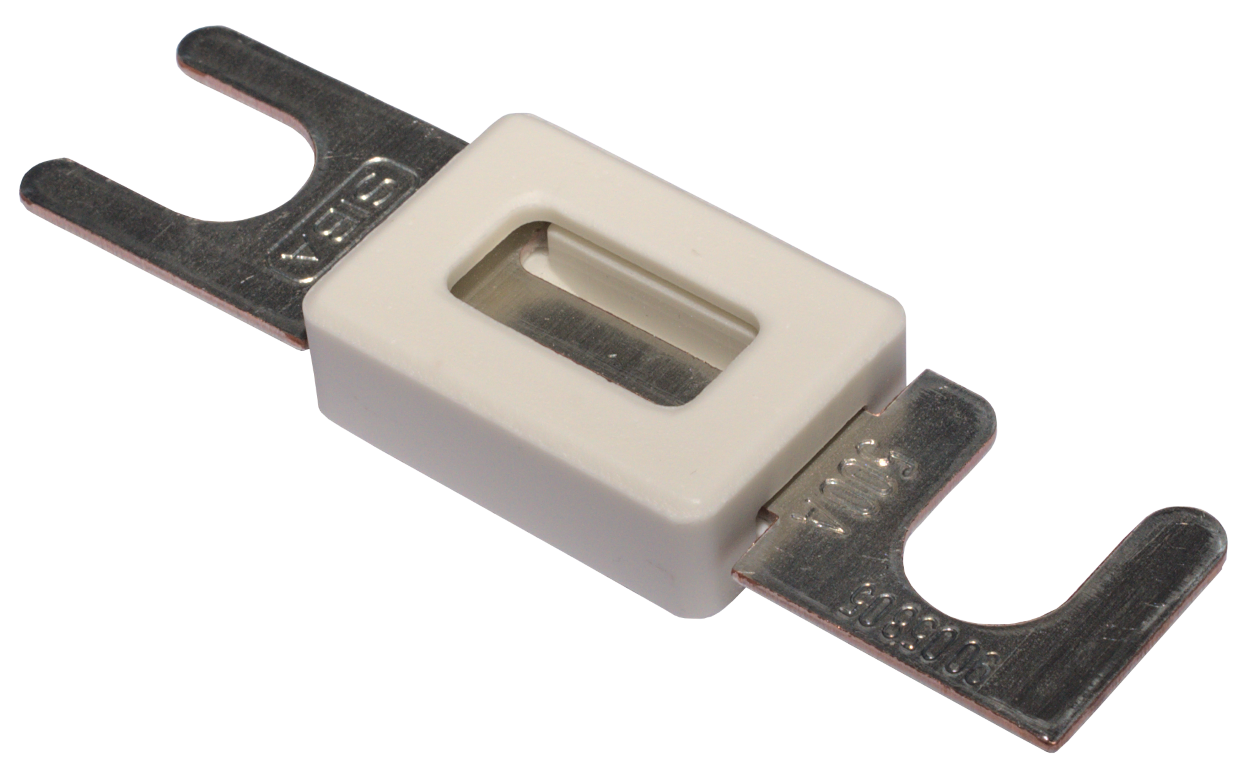
\includegraphics[width=.6\textwidth]{Fotos/kfz_Sicherung.png}
%     \captionof{figure}{KFZ-Sicherung}    
% \end{figure}
